
%%%%%%%%%%%%%%%%%%%%%%%%%%%%%%%%%%%%%%%%%%%%%%%%%%%%%%%%%%%%%%%%%%%%%%%%%%%%
% This will help you in writing your homebook
% Remember that the character % is a comment in latex

% Divide the work you have done in each of the chapters used 
% during the lab lessons in a new chapter, as in the example below, 
% using a coherent title 


% For each chapter you can include :

%-----------------------------
% VHDL file, using the sintax:


	%\begin{listato}
	%\lstinputlisting{./exeMPLE/listato1.vhd}
	%\end{listato}

% the path to the file must be correct, obviously
% Should you have listings written in other languages the method is the 
% same, but the language set up must be changed using a different 
% setting for the command \lstset{language=VHDL} in file homebook.tex 


%-----------------------------
% figures in postcript (ps) or encapsulated postcript (eps)
% format, using the syntax:

%	\begin{figure}[h]
%	\centering
%	\includegraphics[width=9cm]{./cap1/figure1.eps}
%	\caption{Put a caption if you want (didascalia...:)))}
%	\label{put-a-label-for-referring-to-this-picture}	
%	\end{figure}

% the path to the file must be correct, obviously
% you can refer to this picture in any point of your document
% by typing the instruction:

% 	\ref{put-a-label-for-referring-to-this-picture}

% that is using the same label you put in the fiure label
% when you will run the "latex command" an automatic reference to
% this figure with the correct enumeration will be inserted


%-----------------------
% comment in text format (if you are not skilled in latex and don't want to be)
% using the sintax:

	%\begin{verbatim}
	% blablabla 
	%\end{verbatim}

% The verbatimg includes text as it is, as you could write in a normal text file 

% (BETTER) If uou want to write enhancing all the latex possibilities you 
% should add to you text a few commands in some particular cases. 
% In the following you have and example of a few chapters roughtly commented
% and written all in this file: remember that you can saparate
% each chapter in different files (this is always what a latex pro does) 
% and include them using the instruction: \input{./directoryxx/fileyy.tex}


%%%%%%%%%%%%%%%%%%%%%%%%%%%%%%%%%%%%%%%%%%%%%%%%%%%%%%%%%%%%%%%%%%%%%%%%%%%%%%%
%%%%%%%%%%%%%%%%%%%%%%%%%%%%%%%%%%%%%%%%%%%%%%%%%%%%%%%%%%%%%%%%%%%%%%%%%%%%%%%%%
%%%%%%%%%%%%%%%%%%%%%%%%%%%%%%
% Beginning of latex commands
% You can copy this in a new file (e.g. cap1/cap1.tex) and inlcude it here
% using the command : \input{./cap1/cap1.tex}


\chapter[Overview and Features]{Overview and Features}
Our DLX processor is a 5-stage pipelined in-order microprocessor which fully support
general integer instructions and some long latency special integer instructions,
like Multiplication, Division (for both Signed and Unsigned) and Unsigned Square Root.

With maximum forwarding technology, the processor only suffers 1 type of logic hazzaard -- 
Read After Load (RAL).

In order to eliminate or reduce the delay caused by branch, the branch unit is organized
in the 2nd stage (ID) which allows it to make the desition as soon as possible.
Further more, a 2-bit saturating counter based Branch Prediction Unit is embeded in the branch unit to
predict the result of branch in case of Branch After Load (BAL) stall.

\chapter[Structure]{Structure}
The whole DLX microprocessor is organized in 4 parts: the control unit, the datapath,
the instruction RAM and the data RAM. As shown in figure \ref{fig:dlx}
\section[Control Unit]{Control Unit}
Control Unit mainly produces the control words to control the behavior of our microprocessor's Datapath.
It also needs to decide how a stall signal affects the pipeline and whether a branch
is taken or not.

Our microprocessor's Control Unit consists of a Control word generator, a Stall generator and a Branch unit.
As shown in figure \ref{fig:cu}

\subsection[Control Word Generator]{Control Word Generator}
The Control word generator (CwGenerator) is a tiny micro-processor based module with 2 memory levels,
a relocated memory and a microcode memory.

It first looks up a signal called {\it upc2} corresponding to the current instruction in the {\it stage 2 (ID)} and then gets the control
words from the microcode memory based on this {\it upc2} signal. The {\it upc2} can be delayed with offset in each clock cycle,
which makes it {\it upc3}, {\it upc4} and {\it upc5}.

For R-type and F-type instructions, all the control words are the same
except for the part controlling the execution units (ALU, MUL, DIV).
So a single control word that consists of many bits is introduced to solve this sharing problem among R-type
and F-type instructions.

At the end of process, depending on {\it branch flag} and {\it stall flag}, the control words will be masked in
a specific way to form the final control words.

The structure of Control word generator is shown in figure \ref{fig:cg}

\subsection[Stall Generator]{Stall Generator}
The Stall Generator deals with different signals which will lead to stall any stage
of the pipeline. The signals include:

\begin{description}
  \item[RAL] Read After Load, 3rd stage (EXE).
  \item[BPW] Branch Predict Wrong, 3rd stage (EXE).
  \item[JRAL] JR After Load, 2nd stage (ID).
  \item[MUL] Multiplication, 3rd stage (EXE).
  \item[DIV] Division, 3rd stage (EXE).
  \item[SQRT] Square Root, 3rd stage (EXE).
\end{description}

The detail of hazard handling will be covered in Section \ref{ch:hazard}.

For each kind of hazard, we use a F.S.M. and a logic block to determine the behavior of
Datapath, the former is for following clock cycles and the latter is for the current clock
cycle. Finally, the {\it stall\_flag} signal is produced by performing OR operation between
the resulting signals obtained from these blocks.

The structure of Stall generator is shown in figure \ref{fig:sg}

\subsection[Branch]{Branch}
The Branch Unit calculates the result of branch instructions by checking the value
of the invoving register. It will make predictions when the value of this register
is not ready.

The detail of Branch After Load (BAL) hazard will be covered in section \ref{ch:hazard}. And the
detail of Branch Prediction will be covered in section \ref{ch:bpu}

The structure of Branch unit is shown in figure \ref{fig:br}

\section[Datapath]{Datapath}

\subsection[IF]{IF}
\subsection[ID]{ID}
\subsection[EXE]{EXE}
\subsection[MEM]{MEM}
\subsection[WB]{WB}
\subsection[EXTRA]{EXTRA}

\section[RAM]{RAM}
The Instruction RAM and Data RAM are implemented like register files. They performs
either a read operation or a write operation within a single clock cycle without
data missing.

The structure of IRAM is shown in figure \ref{fig:ir} and the structure of DRAM
is shown in figure \ref{fig:dr}. 

\section[Hazard Handling]{Hazard Handling}
\label{ch:hazard}
\subsection[Forwarding]{Forwarding}
Many kinds of Hazards can be eliminated by introducing forwarding. Our forwarding
unit (Fwd2) is a 2-stage forwarding module with unwanted match indication.

The forwarding unit recieves the value of the current stage, the feedback value
of the next stage and the feedback value of the next next stage. It also receives
enable signals to indicate the possiblity to perform the match operation with each
feedback value. Two additional inputs {\it dirty\_f and dirty\_ff} are used to
indicate the avalability of the feedback values. The output will be a value choosen from these
3 values based on their addresses and enable signals. If a match is labeled with
"dirty match", the corresponding output signal will be '1' in order to notify other
components that the output is not correct. The "dirty match" will usually lead to
a stall process.

The structure of Forwarding unit is shown in figure \ref{fig:fwd}

\subsection[Read After Load (RAL)]{Read After Load (RAL)}
The Read After Load (RAL) hazard arises when the value of a register is needed by
one of the two operands of execution units while the same register should be
updated by a Load instruction which is 1 clock cycle
in front. Since the value will not be available until the end of stage 4 (MEM), even
with 2 stage forwarding, the problem still exists.

To solve the problem, we need to stall the pipeline. The sequence of stall flag
is shown in talbe \ref{tab:stall_ral}.

\begin{table}[!ht]
\centering
\caption{Stall Flag for RAL}
\label{tab:stall_ral}
\begin{tabular}{|l|l|l|l|l|}
\hline
IF & ID & EXE & MEM & WB \\
\hline
1  & 1  & 1  & 0  & 0\\
0  & 0  & 0  & 1  & 0\\
0  & 0  & 0  & 0  & 1\\
0  & 0  & 0  & 0  & 0 \\
\hline
\end{tabular}
\end{table}

Unfortunately, the solution is still not perfect. There is a satuation when one
operand (assuming A) is regularly matched with a double-forwarding feedback (from
stage 5) while the other operand (assuming B) triggers a RAL stall by dirty matching
the feedback of stage 4. After the 1 clock cycle stall, the value of B becomes correct,
but the value of A becomes wrong since forwarding is not valid for A at the new clock cycle.
Therefore, the value for A and B shoud be kept for 1 clock cycle. In case of RAL stall happens, the
kept correct value for the other operand can be restored if needed.

\subsection[JR After Load (JRAL)]{JR After Load (JRAL)}
JR After Load (JRAL) hazard happens when a JR or JALR instruction follows a Load
instruction which will update the register requested by JR/JALR instruction. Similar
to RAL hazard, it will trigger a stall for 1 clock cycle, the stall flag sequence is
shown in table \ref{tab:stall_jral}.

\begin{table}[!ht]
\centering
\caption{Stall Flag for JRAL}
\label{tab:stall_jral}
\begin{tabular}{|l|l|l|l|l|}
\hline
IF & ID & EXE & MEM & WB \\
\hline
1  & 1  & 0  & 0  & 0\\
0  & 0  & 1  & 0  & 0\\
0  & 0  & 0  & 1  & 0\\
0  & 0  & 0  & 0  & 1\\
0  & 0  & 0  & 0  & 0 \\
\hline
\end{tabular}
\end{table}

\subsection[Branch After Load (BAL)]{Branch After Load (BAL)}
Similar to JRAL, Branch After Load hazard should request a pipeline stall too. However,
the problem is solved by introducing the Branch Prediction Unit. The
detail of Branch Prediction will be covered in section \ref{ch:bpu}

\subsection[Store After After Write (SAAW)]{Store After After Write (SAAW)}
A Store After After Write hazard happens when a Store instruction is 2 stages later than
an instruction writing to the same register that requested by the Store instructions.
This will becomes a problem when there are only 5 stages. The Store instruction which
is in the stage 4 cannot get the double-forwarding feedback since there is no stage 6.
To solve the problem, we add a stage 6 (EXTRA) which simply delays the value of stage 5,
and feedback to stage 4 in case of SAAW.

\subsection[Long Latency Execution]{Long Latency Execution}
Our DLX processor support some long latency execution like DIV, MUL and SQRT. These
operation can not be completed within 1 clock cycle. While executing these instructions,
the stage 3 will be occupied for a long time and the pipeline should be stalled.
The stall flag sequence is shown in table \ref{tab:stall_lle}.

\begin{table}[!ht]
\centering
\caption{Stall Flag for Long Latency Execution}
\label{tab:stall_lle}
\begin{tabular}{|l|l|l|l|l|}
\hline
IF & ID & EXE & MEM & WB \\
\hline
1  & 1  & 1  & 0  & 0\\
1  & 1  & 1  & 1  & 0\\
1  & 1  & 1  & 1  & 1\\
\hline
\multicolumn{5}{ |c| }{....}\\
\hline
1  & 1  & 1  & 1  & 1\\
0  & 0  & 0  & 1  & 1\\
0  & 0  & 0  & 0  & 1\\
0  & 0  & 0  & 0  & 0\\
\hline
\end{tabular}
\end{table}

\section[Branch Prediction]{Branch Predition}
\label{ch:bpu}
The information for each branch prediction is stored inside a branch history table (BHT).

The BHT is organized like a direct-mapped cache. Each entry contains 2 fields:
TAG and VALUE. TAG is determined by the first part of branch address (Default 25 bits) and VALUE
is the current 2-bit state of the branch instruction. The index of each entry is
determined by the middle part of address (Default 5 bits).

\begin{table}[!ht]
\centering
\caption{Address of branch instruction}
\label{tab:bpu_addr}
\begin{tabular}{|l|l|l|}
\hline
TAG (25 bits) & INDEX (5 bits) & Always 0 for any instruction (2 bits) \\
\hline
\end{tabular}
\end{table}

\begin{table}[!ht]
\centering
\caption{BHT structure}
\label{tab:bpu_bht}
\begin{tabular}{|l|l|}
\hline
\multicolumn{2}{ |c| }{ }\\
\hline
\multicolumn{2}{ |c| }{....}\\
\hline
TAG (25 bits) & VALUE (2 bits) \\
\hline
\multicolumn{2}{ |c| }{....}\\
\hline
\multicolumn{2}{ |c| }{ }\\
\hline
\end{tabular}
\end{table}

\begin{table}[!ht]
\centering
\caption{VALUE Meaning}
\label{tab:bpu_value}
\begin{tabular}{|l|l|}
\hline
00 & Strongly not taken \\
01 & Weakly not taken \\
10 & Weakly taken \\
11 & Strongly taken \\
\hline
\end{tabular}
\end{table}

The branch prediction can be devided into 2 phases: prediction phase and verification phase.

During the prediction phase (ID stage), it look up the BHT by index, compare the TAG and get the VALUE.
Based on VALUE, it predict whether the branch will take or not. If the TAG doesn't match,
the entry will be replaced with the new TAG with VALUE="00".

During the verification phase (EXE stage), it check whether the previous prediction
is correct or not. and update the VALUE area according the rule shown in figure \ref{fig:bpu_rule}
\begin{figure}[Ht]
    \centering
    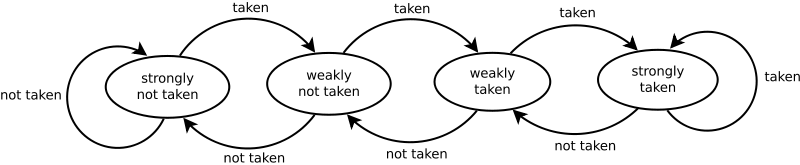
\includegraphics[width=0.8\textwidth]{fig/bpu_rule.png}
    \caption{BHT VALUE update rule}
    \label{fig:bpu_rule}
\end{figure}

\section[Long Latency Instructions]{Long Latency Instructions}
\subsection[Multiplication]{Multiplication}
The structure of Multiplier is shown in figure \ref{fig:mul}.

\subsubsection[MULT]{MULT}
Signed multiplication is realized with booth's algorithm, completed within 8 clock cycles.

With properly encoding the output of Booth Encoder and introducing of Adder/Substractor,
we reduced the complexity of multiplexer and removed the substractors needed by calculating -a and -2a.
The encoding rules are shown in table \ref{tab:booth_enc}.

\begin{table}[!ht]
\centering
\caption{Booth Encoder Output}
\label{tab:booth_enc}
\begin{tabular}{|l|l|l|}
\hline
BIT2 & ZERO bit & "0" if we need to choose "0", otherwise "1"\\
\hline
BIT1 & SIGN bit & "0" if we need to choose +a or +2a, otherwise "1"\\
\hline
BIT0 & DOUBLE bit & "0" if we need to choose +a or -a, otherwise "1"\\
\hline
\end{tabular}
\end{table}

\subsubsection[MULTU]{MULTU}
Unsigned multiplication is a standard unsigned multiplication with some modification
in inputs and output.

Let's take a 4-bit unsigned multiplication as an example:

\begin{align*}
&[A_3|A_2|A_1|A_0] \times [B_3|B_2|B_1|B_0]\\
=&[A_3B_3|A_3B_2+A_2B_3|A_3B_1+A_2B_2+A_1B_3|A_3B_0+A_2B_1+A_1B_2+A_0B_3|\\
 &A_2B_0+A_1B_1+A_0B_2|A_1B_0+A_0B_1|A_0B_0]
\end{align*}

The result can be further divided into several parts.

\begin{align*}
&[A_3|A_2|A_1|A_0] \times [B_3|B_2|B_1|B_0]\\
=&[A_3B_3|A_3B_2+A_2B_3|A_3B_1+A_2B_2+A_1B_3|A_3B_0+A_2B_1+A_1B_2+A_0B_3|\\
 &A_2B_0+A_1B_1+A_0B_2|A_1B_0+A_0B_1|A_0B_0]\\
=&[A_2B_2|A_1B_2+A_1B_2|A_2B_0+A_1B_1+A_0B_2|A_1B_0+A_0B_1|A_0B_0]+\\
 &([A_3|A_2|A_1|A_0]B_3+[B_3|B_2|B_1|B_0]A_3-[A_3B_3|0|0|0]) << 3\\
=&[0|A_2|A_1|A_0] \times [0|B_2|B_1|B_0]+\\
 &([A_3|A_2|A_1|A_0]B_3+[B_3|B_2|B_1|B_0]A_3-[A_3B_3|0|0|0]) << 3
\end{align*}

With this equation, we can transfer a 4-bit unsigned multiplication to 4-bit signed multiplication
of 2 positive operands. The result should be adjusted by adding $([A_3|A_2|A_1|A_0]B_3+[B_3|B_2|B_1|B_0]A_3-[A_3B_3|0|0|0]) << 3$.

In summary, an unsigned multiplication can be convert to a signed multiplication by
performing some modification on inputs and output. So the total latency for a multiplication
will be 10 clock cycles, which include 1 clock cycle for input adjustment, 8 clock cycles
for signed multiplication and 1 clock cycle for output adjustment.

\subsection[Division]{Division}
The structure of Divider is shown in figure \ref{fig:div}.

\subsubsection[DIVU]{DIVU}
The core part which performs unsigned division is based on the
Non-Restoring Division algorithm, completed within 32 clock cycles.

The control part of the divider is a F.S.M.

\subsubsection[DIV]{DIV}
The signed division is based on the unsigned division with properly adjust the inputs
and output.

If we define that {\bf the sign of the reminder should be the same as the dividend},
we can conclude that {\bf the absolute value of quotient is the same for both signed and
unsigned division}. Therefore, we can get the result of signed division by only adjust
the sign of the quotient calculated by unsigned division. Whether to perform the
adjustment of output depends on the signs of both dividend and divisor. The rules
are shown in table \ref{tab:div_sign}.

\begin{table}[!ht]
\centering
\caption{Sign adjust rules}
\label{tab:div_sign}
\begin{tabular}{|c|c|c|}
\hline
Dividend & Divisor & Output Adjust\\
\hline
+ & + & No\\
+ & - & Yes\\
- & + & Yes\\
- & - & No\\
\hline
\end{tabular}
\end{table}

In summary, a signed division can be convert to an unsigned multiplication by
performing some modification on inputs and output. So the total latency for a division
will be 34 clock cycles, which include 1 clock cycle for input adjustment, 32 clock cycles
for unsigned division and 1 clock cycle for output adjustment.

\subsection[Square Root]{Square Root}
Only unsigned square root exists in real domain.

A Restoring Square root algorithm is based on equation $(a+b)^2=a^2+2ab+b^2$. For binary
digits, if we assuming $SQRT(X)=[ab]$, with b equals either 1 or 0. We can
get:

\begin{align*}
X & >= (a\cdot 2^1+b)^2\\
  & = (a\cdot 2^1)^2+2\cdot a\cdot 2^1 \cdot b + b^2\\
  & = 4a + 4(ab) + b^2\\
So,\\
R_{n} & = (X-4a)\\
  & >= 4(ab) + b^2\\
We\ set:\\
R_{n+1}^{es} &= R_{n} - [4(ab) + b^2]
\end{align*}

Therefore, let's guess b=1:
\begin{align*}
R_{n+1}^{es} &= R_{n} - [4a + 1]
\end{align*}

If $R_{n-1}^{es}>=0$, the guess is correct; otherwise, the guess is wrong, we need
restore $R_{n+1}=R_{n}$.

The Non-Restoring method is similar. Instead of restoring the reminder, we compensate
the wrong guess in the next substraction.

Therefore, we can use the same hardware resources of division with a little modification. The reminder
will be appended 01 or 11 instead of left shift 1 bit in each clock cycle and the position of divisor
will be replaced by shifted intermediate quotient.

An example is shown in table \ref{tab:sqrt}.

\begin{table}[!ht]
\centering
\caption{SQRT example}
\label{tab:sqrt}
\begin{tabular}{rrrrr l}
  &  1 &  0 &  0 &  1 & \\
\hline
) & 01 & 01 & 11 & 01 & Positive\\
- & 01 &    &    &    & Since positive, append 01 and perform SUB\\
\hline
  & 00 & 01 &    &    & Positive, append Q with 1, Now Q=1\\
- &  1 & 01 &    &    & Since positive, append 01 and perform SUB\\
\hline
  & 11 & 00 & 11 &    & Negative, append Q with 0, Now Q=10\\
+ &    & 10 & 11 &    & Since negative, append 11 and perform ADD\\
\hline
  & 11 & 11 & 10 & 01 & Negative, append Q with 0, Now Q=100\\
+ &    &  1 & 00 & 11 & Since negative, append 11 and perform ADD\\
\hline
  &    &    & 11 & 00 & Positive, append Q with 1, Now Q=1001\\
\end{tabular}
\end{table}


\chapter[Synthesis and Optimization]{Synthesis and Optimization}
For the synthesis part, we only optimized the delay with time constrain $clock=2.5$.
The critical path is in the stage 2 which is used to generate the jump address. This
is because:

\begin{description}
  \item The relative jump address will ADD to the next pc counter, which will take time.
  \item The register file works at the FALLING edge of clock.
  \item The branch unit especially the branch prediction unit works after it gets the register value from the register file.
  \item In case of wrong prediction happens, the final jump address will be changed.
\end{description}

In summary, the synthesis result is listed in table \ref{tab:syn}.
\begin{table}[!ht]
\centering
\caption{Synthesis Result}
\label{tab:syn}
\begin{tabular}{|c|c|c|}
\hline
Timing(Arrive Time) & Before Optimization & 3.27 \\
\hline
Timing(Arrive Time) & After Optimization & 2.03 \\
\hline
Area & Before Optimization & 30520.839844 \\
\hline
Area & After Optimization & 31421.783203 \\
\hline
\end{tabular}
\end{table}

\chapter[Appendix]{Appendix}
\section[Diagram]{Diagram}
\begin{figure}[Ht]
    \centering
    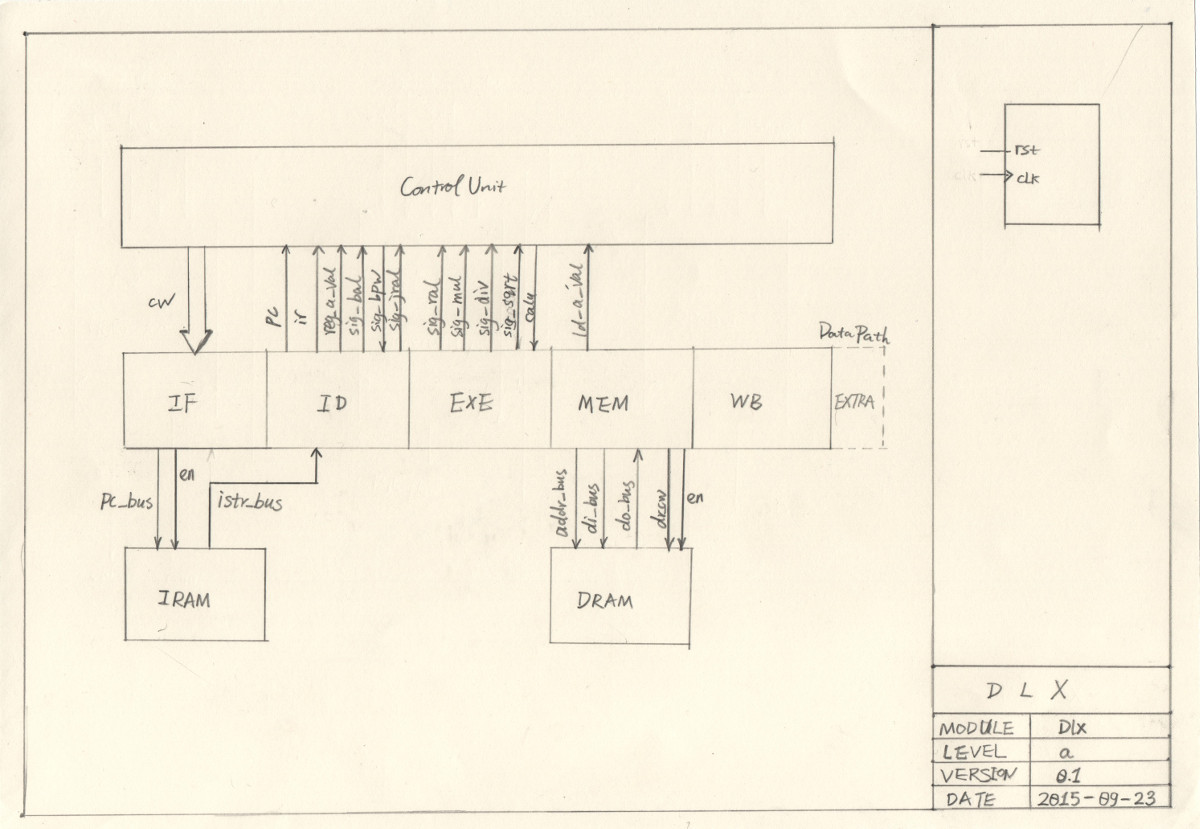
\includegraphics[width=0.8\textwidth]{fig/dlx.jpg}
    \caption{DLX overall structure}
    \label{fig:dlx}
\end{figure}
\begin{figure}[Ht]
    \centering
    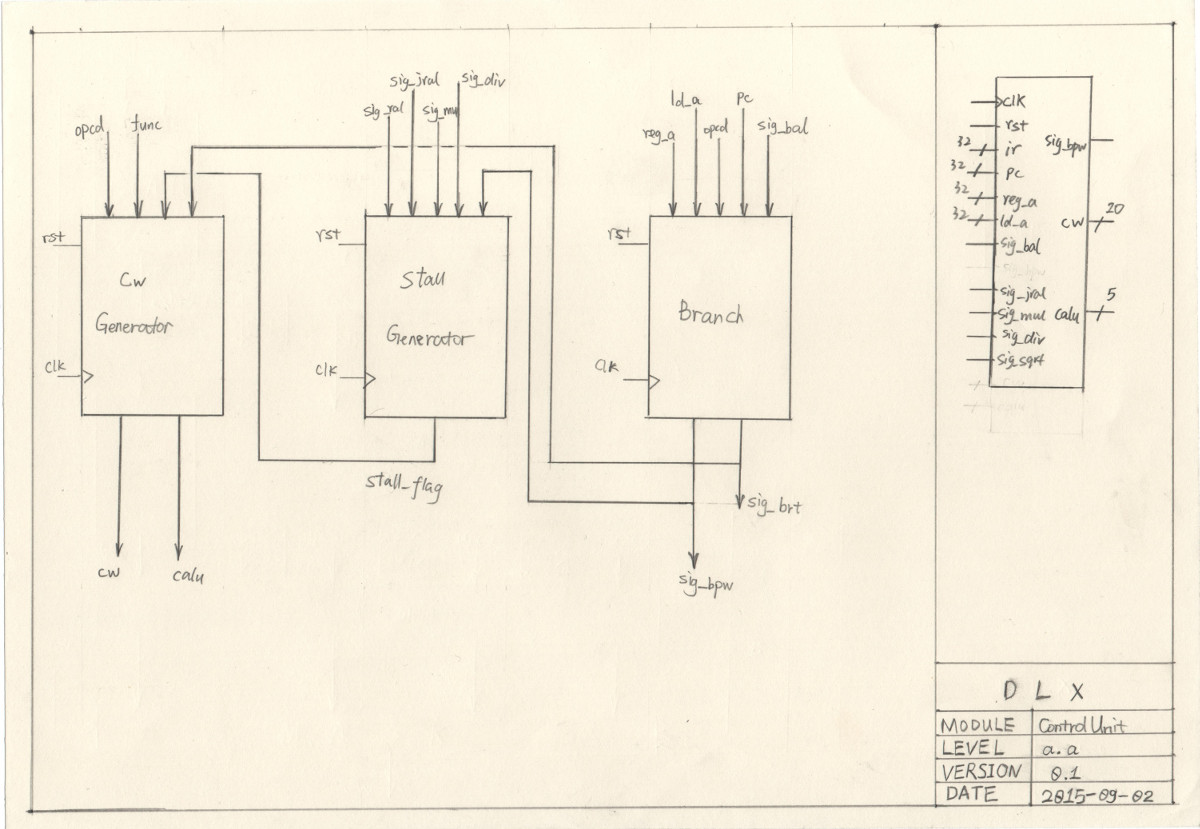
\includegraphics[width=0.8\textwidth]{fig/cu.jpg}
    \caption{Control Unit}
    \label{fig:cu}
\end{figure}
\begin{figure}[Ht]
    \centering
    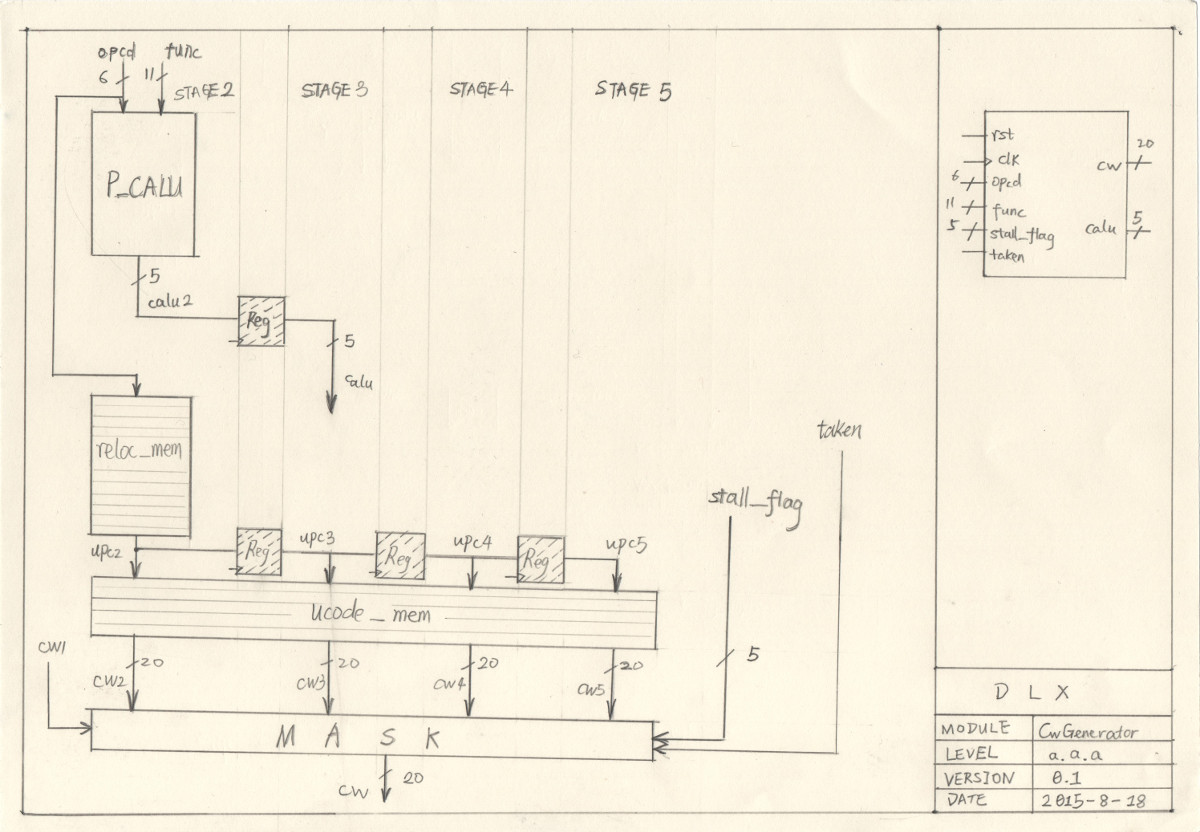
\includegraphics[width=0.8\textwidth]{fig/cg.jpg}
    \caption{Control Word Generator}
    \label{fig:cg}
\end{figure}
\begin{figure}[Ht]
    \centering
    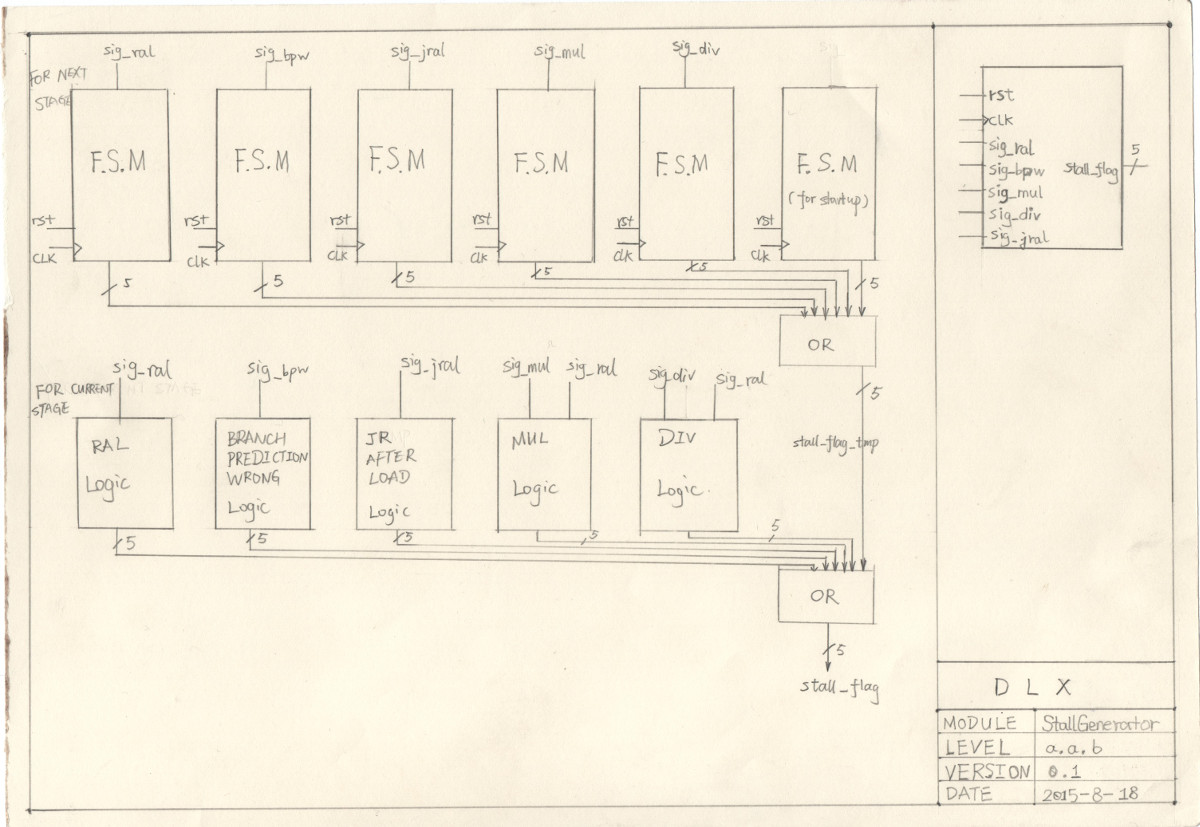
\includegraphics[width=0.8\textwidth]{fig/sg.jpg}
    \caption{Stall Generator}
    \label{fig:sg}
\end{figure}
\begin{figure}[Ht]
    \centering
    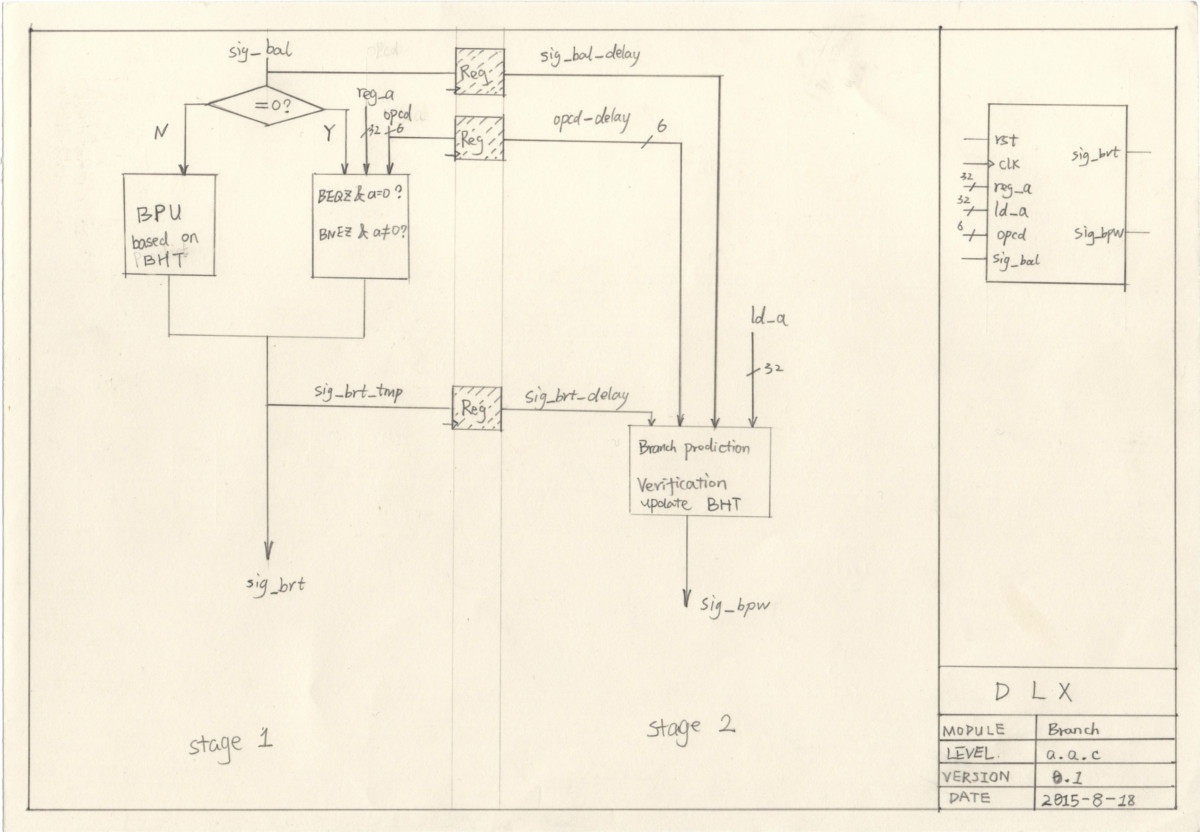
\includegraphics[width=0.8\textwidth]{fig/br.jpg}
    \caption{Branch Unit}
    \label{fig:br}
\end{figure}
\begin{figure}[Ht]
    \centering
    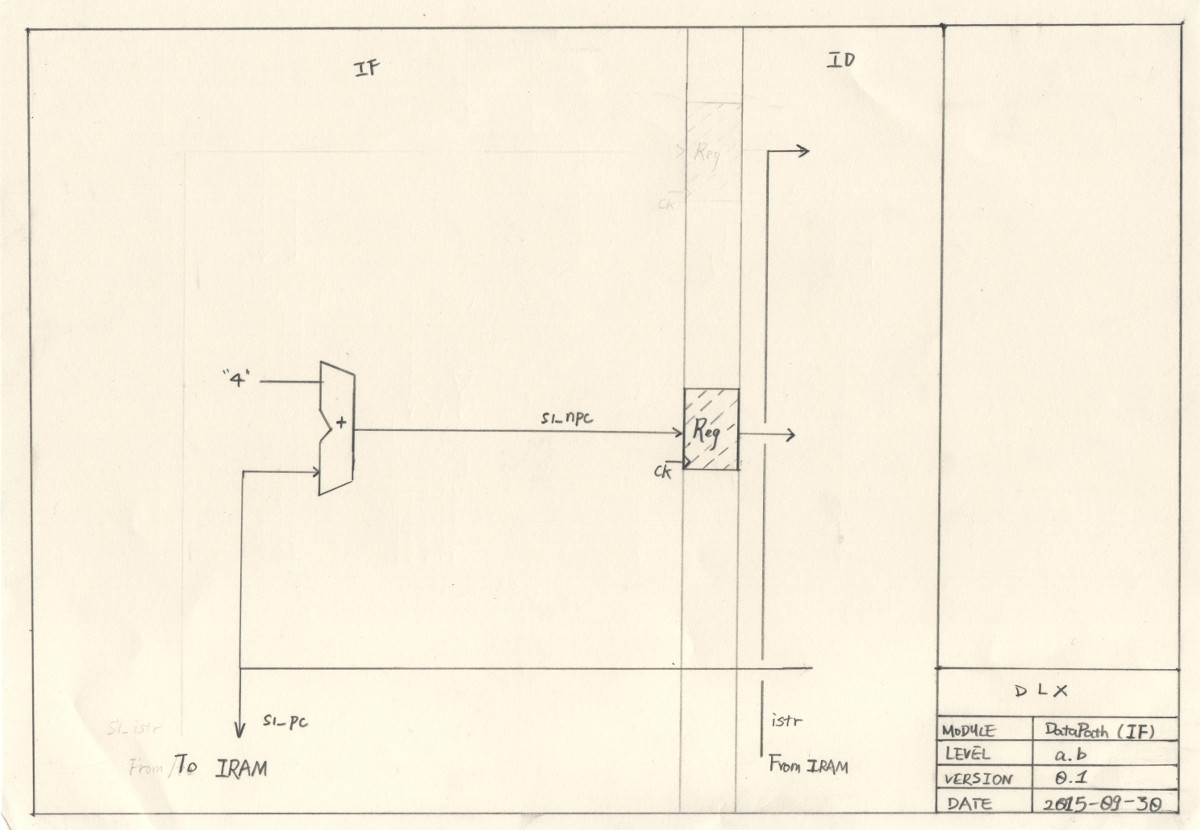
\includegraphics[width=0.8\textwidth]{fig/dp1.jpg}
    \caption{Datapath (IF)}
    \label{fig:dp1}
\end{figure}
\begin{figure}[Ht]
    \centering
    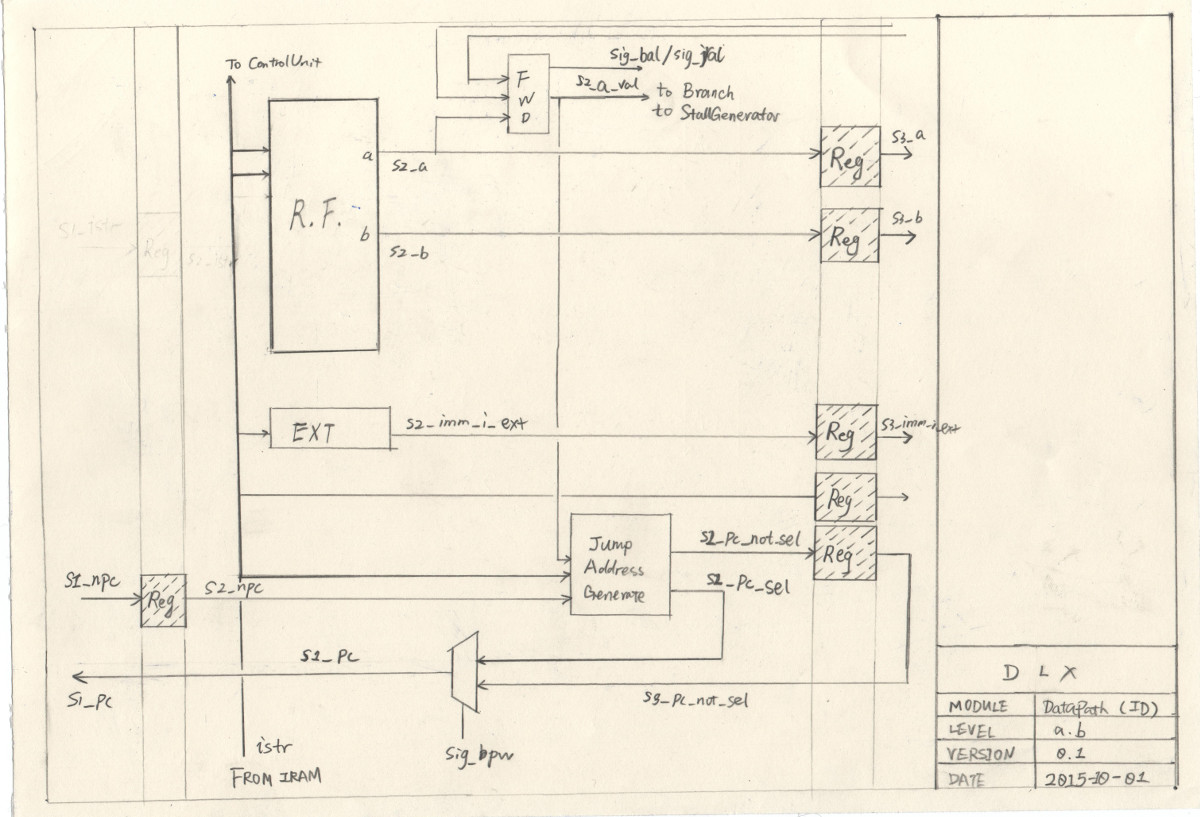
\includegraphics[width=0.8\textwidth]{fig/dp2.jpg}
    \caption{Datapath (ID)}
    \label{fig:dp2}
\end{figure}
\begin{figure}[Ht]
    \centering
    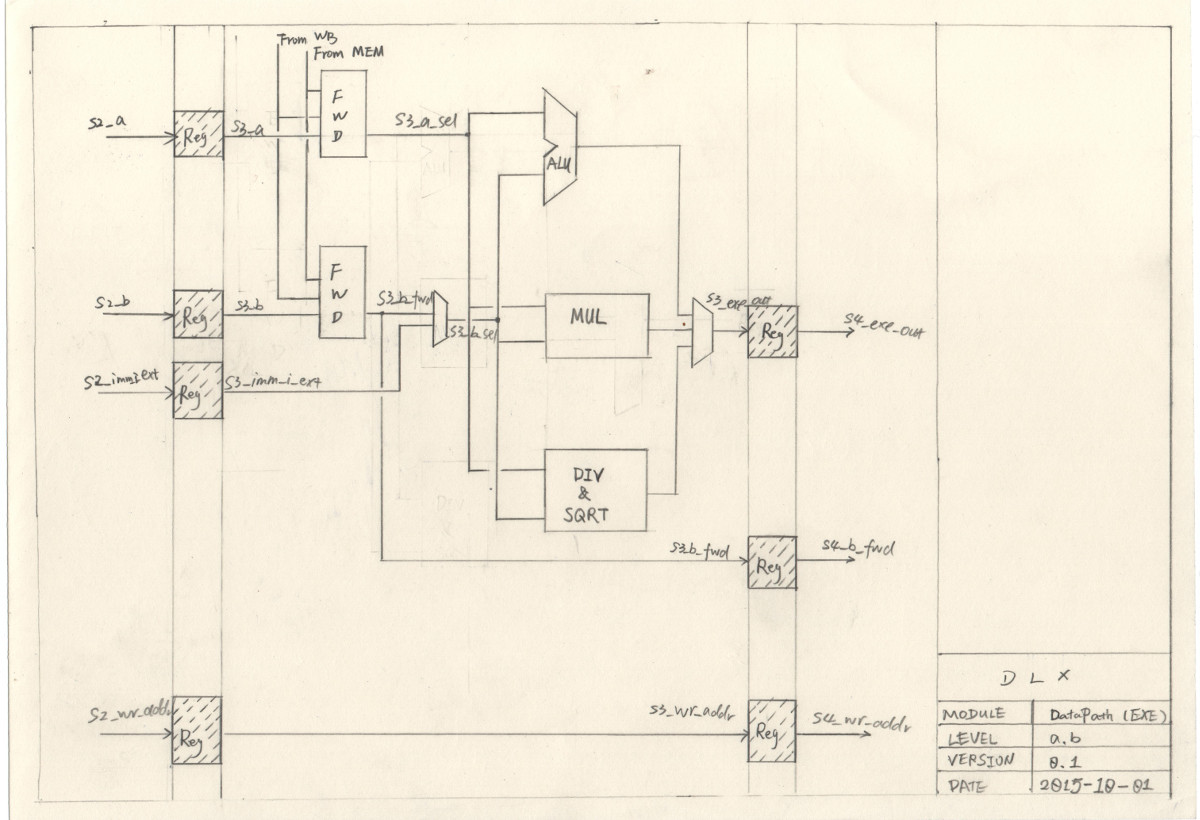
\includegraphics[width=0.8\textwidth]{fig/dp3.jpg}
    \caption{Datapath (EXE)}
    \label{fig:dp3}
\end{figure}
\begin{figure}[Ht]
    \centering
    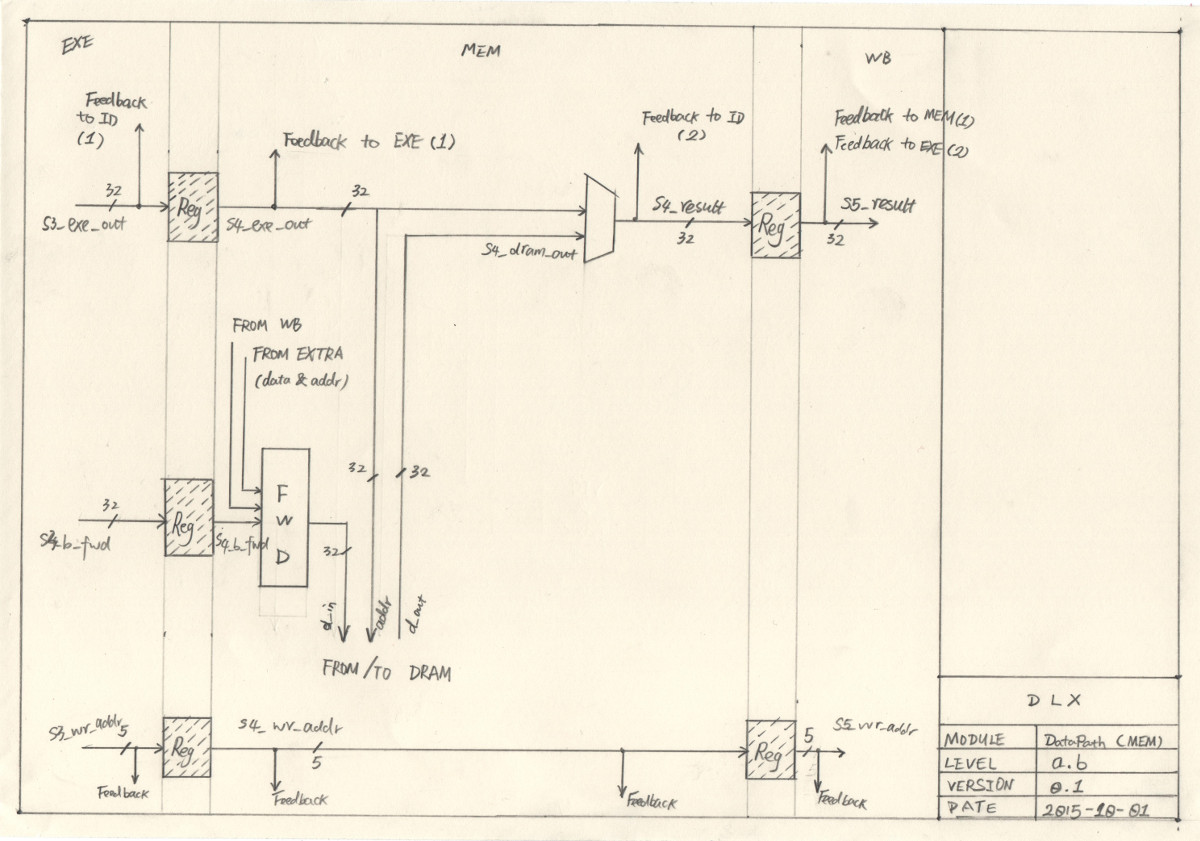
\includegraphics[width=0.8\textwidth]{fig/dp4.jpg}
    \caption{Datapath (MEM)}
    \label{fig:dp4}
\end{figure}
\begin{figure}[Ht]
    \centering
    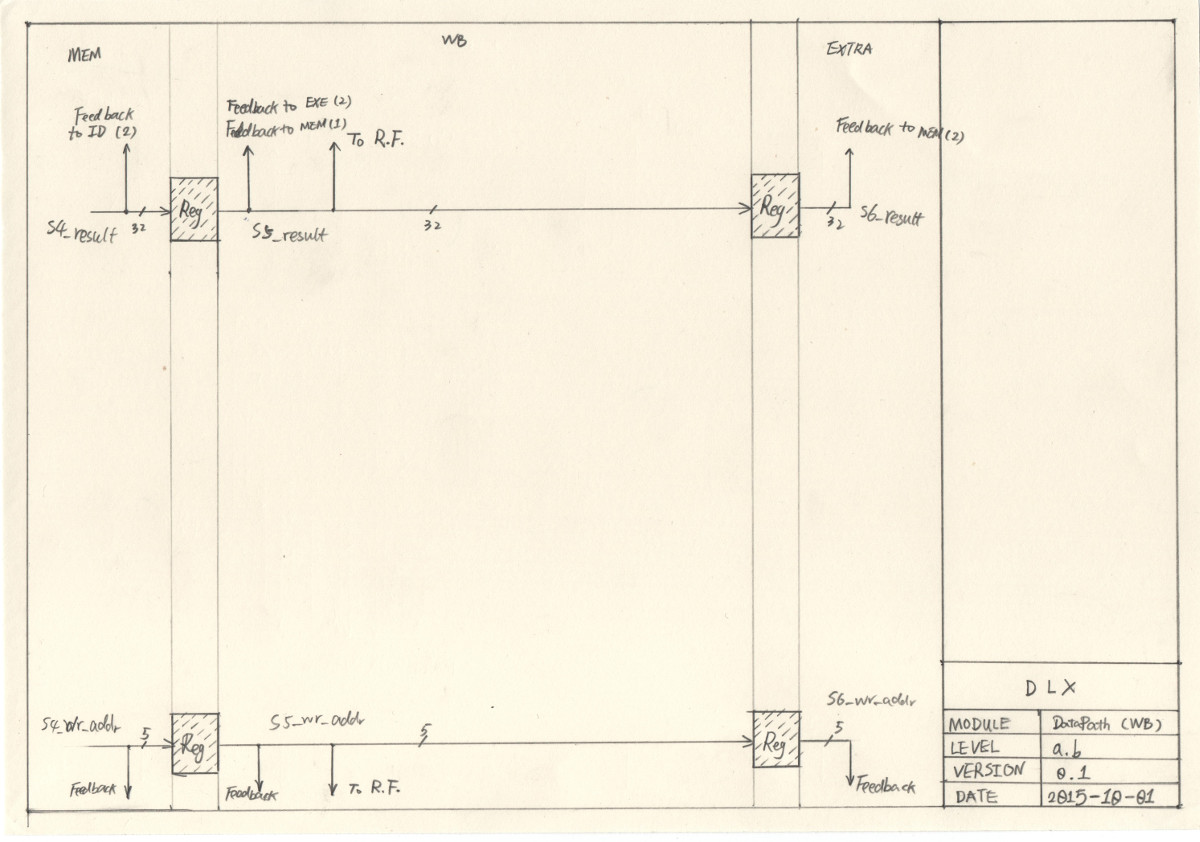
\includegraphics[width=0.8\textwidth]{fig/dp5.jpg}
    \caption{Datapath (WB)}
    \label{fig:dp5}
\end{figure}
\begin{figure}[Ht]
    \centering
    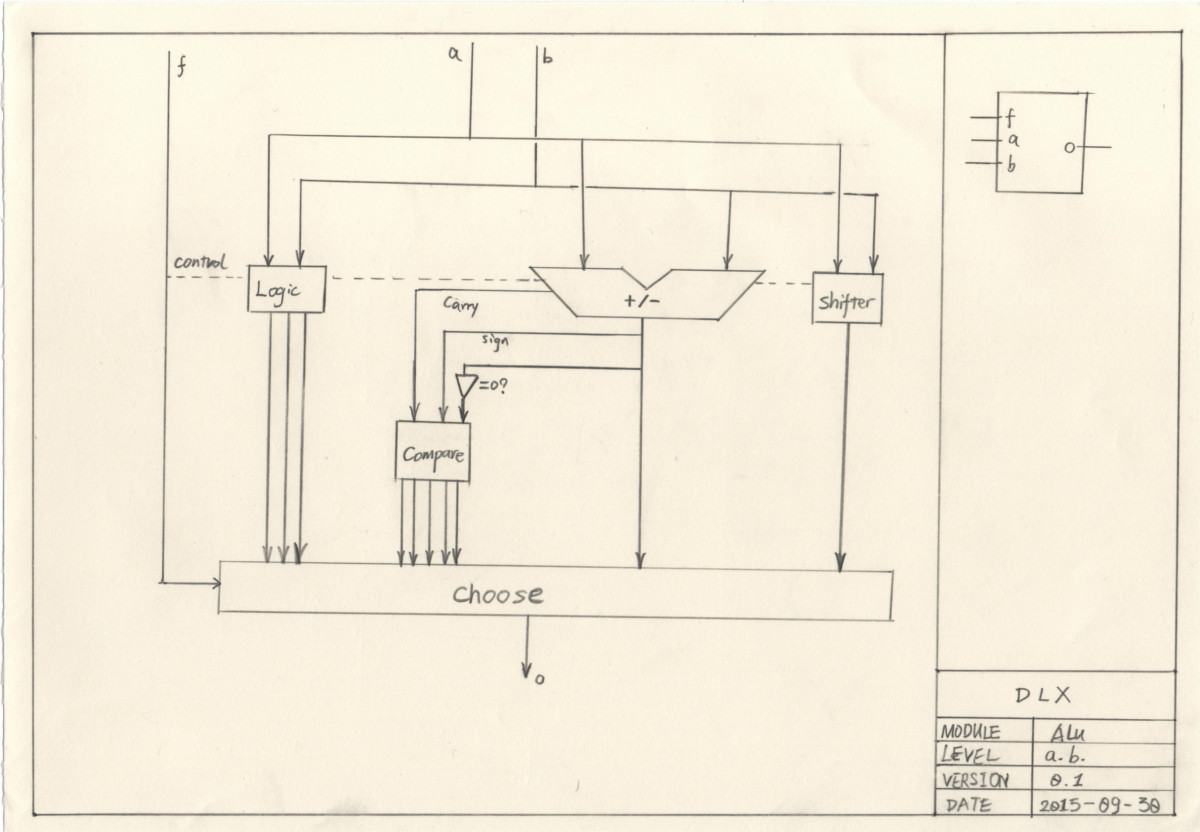
\includegraphics[width=0.8\textwidth]{fig/alu.jpg}
    \caption{ALU}
    \label{fig:alu}
\end{figure}
\begin{figure}[Ht]
    \centering
    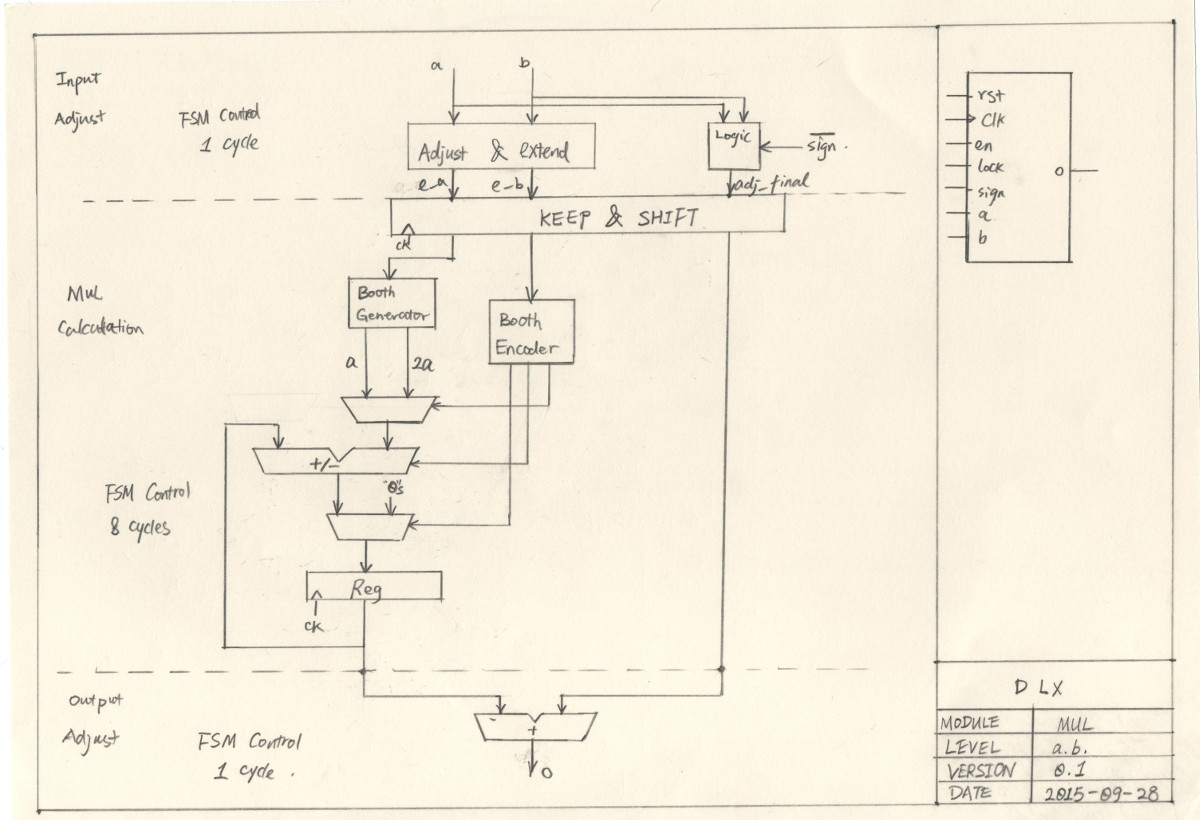
\includegraphics[width=0.8\textwidth]{fig/mul.jpg}
    \caption{Multiplier}
    \label{fig:mul}
\end{figure}
\begin{figure}[Ht]
    \centering
    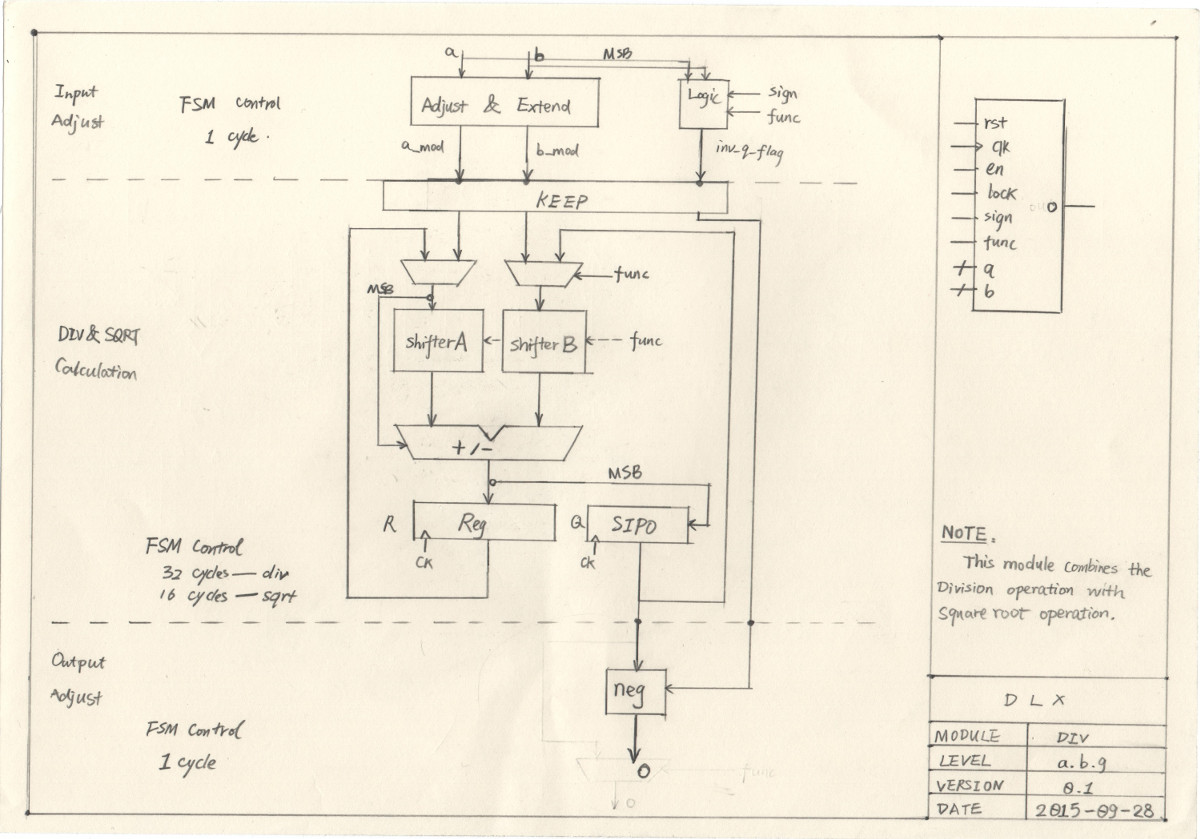
\includegraphics[width=0.8\textwidth]{fig/div.jpg}
    \caption{Divider and SQRT unit}
    \label{fig:div}
\end{figure}
\begin{figure}[Ht]
    \centering
    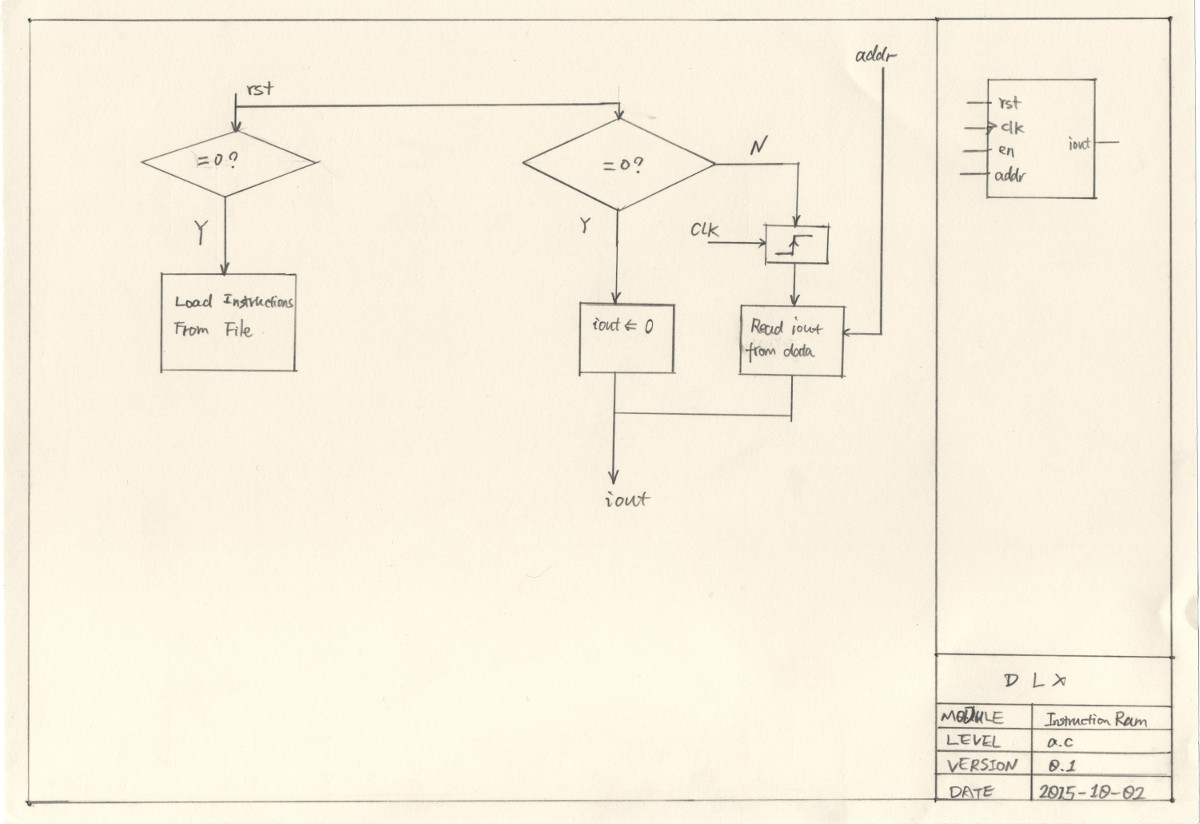
\includegraphics[width=0.8\textwidth]{fig/ir.jpg}
    \caption{Instruction RAM}
    \label{fig:ir}
\end{figure}
\begin{figure}[Ht]
    \centering
    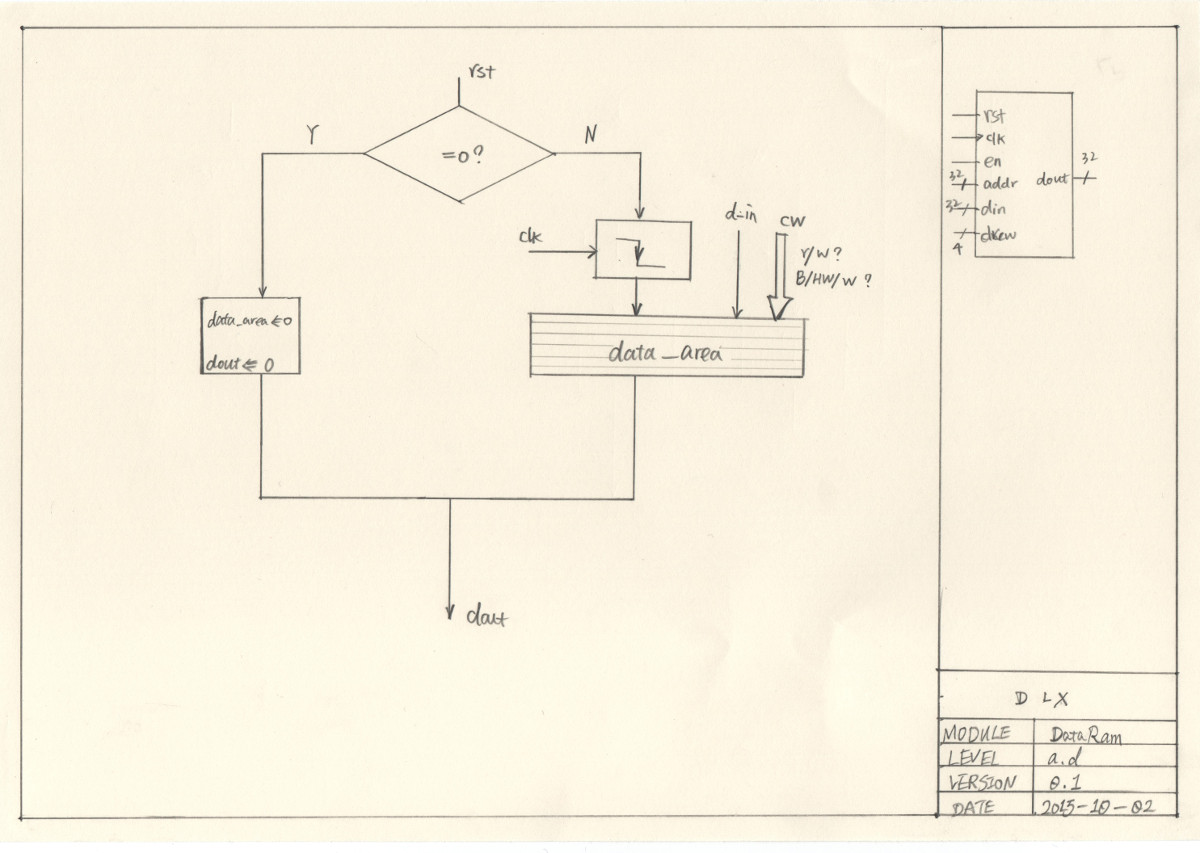
\includegraphics[width=0.8\textwidth]{fig/dr.jpg}
    \caption{Data RAM}
    \label{fig:dr}
\end{figure}
\begin{figure}[Ht]
    \centering
    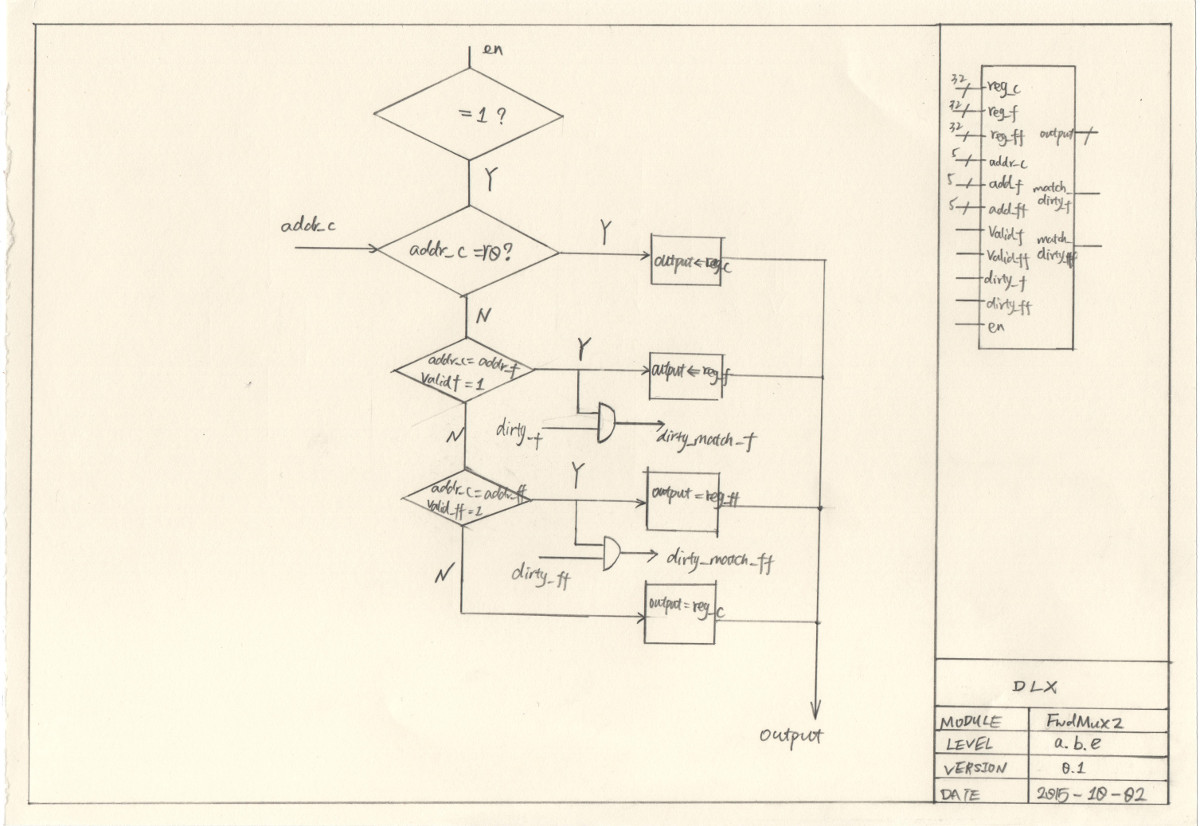
\includegraphics[width=0.8\textwidth]{fig/fwd.jpg}
    \caption{Forwarding Unit}
    \label{fig:fwd}
\end{figure}

